\documentclass{report}
\usepackage[utf8]{inputenc}
\usepackage[ngerman]{babel}
\usepackage{graphicx}
\usepackage{float}
\usepackage{commath}
\usepackage{hyperref}


\let\emph\relax % there's no \RedeclareTextFontCommand
\DeclareTextFontCommand{\emph}{\bfseries}



\title{Einführung in die Hochfrequenz-Übertragungstechnik}
\author{Jonas Otto}
\date{März 2020}

\begin{document}

\tableofcontents
\maketitle

\chapter{Wellen}

\chapter{Leitungen}
\begin{figure}[H]
    \centering
    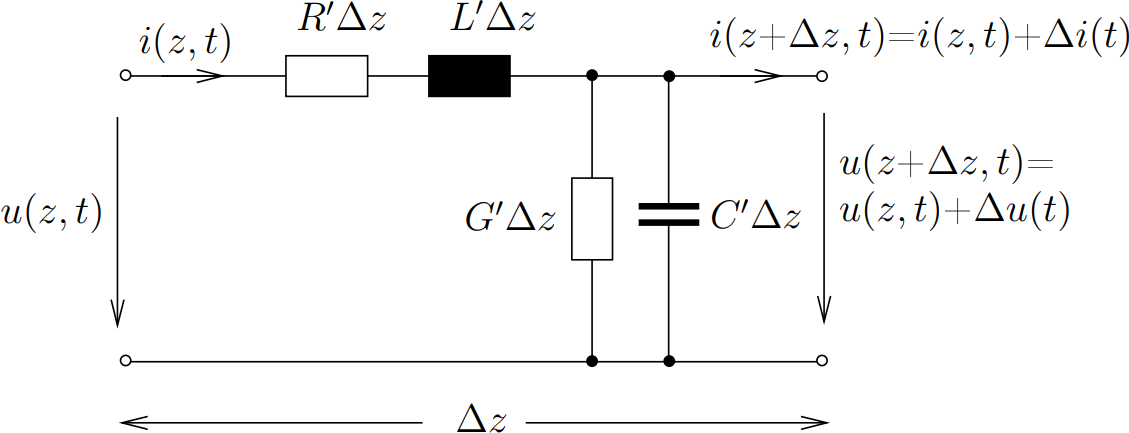
\includegraphics[width=\textwidth]{images/leitung.png}
    \caption{Infinitesimal kurzes TEM-Leitungsstück.}
\end{figure}

\section{Parameter Leitung}
Infinitesimales Leitungsstück kann mit Ersatzschaltbild mit Bauteilgrößen dargestellt werden:
\begin{description}
    \item[$R'$] \emph{Widerstandbelag}
    \item[$L'$] \emph{Induktivitätsbelag}
    \item[$G'$] \emph{Leitwertsbelag}
    \item[$C'$] \emph{Kapazitätsbelag}
\end{description}
Jeweils pro Längeneinheit.

Mittels komplexer Wechselstromrechnung und Kirchhoffschen Gesetzen ergibt sich die \emph{Telegrafengleichung}:
\begin{equation}
    \tag{Telegrafengleichung}
    \od[2]{\underline{U}}{z} = \underline{\gamma^2}\underline{U}
    \label{eqn:Telegraf}
\end{equation}
mit
\begin{equation}
    \tag{Gamma}
    \underline{\gamma} := \sqrt{\left(R'+j\omega L'\right)\left(G'+j\omega C'\right)} = \alpha + j\beta = j\underline{k}_z
\end{equation}

Die Spannung lässt sich als Überlagerung einer hin- und zurücklaufenden Welle interpretieren:
\begin{equation}
    \underline{U}(z)=\underline{U}_h(z)+\underline{U}_r(z) = \underline{U}_{h0} e^{-\underline{\gamma}z}+\underline{U}_{r0} e^{\underline{\gamma}}z
\label{eqn:u-uberlagerung}
\end{equation}

$\implies$ Der \emph{Ausbreitungskoeffizient $\gamma$} enthält alle Leitungsparameter.
Bei verlustloser Leitung besteht dies nur aus dem \emph{Phasenkoeffizient $\beta$}, da dann der \emph{Dämpfungskoeffizient $\alpha$} $= 0$ ist.

Damit lässt sich der \emph{Wellenwiderstand $Z_0$} berechnen:
\begin{equation}
    \underline{Z}_0 := \frac{R'+j\omega L'}{\underline{\gamma}} = \sqrt{\frac{R'+j\omega L'}{G'+j\omega C'}}
\end{equation}



\section{Leitung mit Abschlussimpedanz}
\begin{figure}[H]
    \centering
    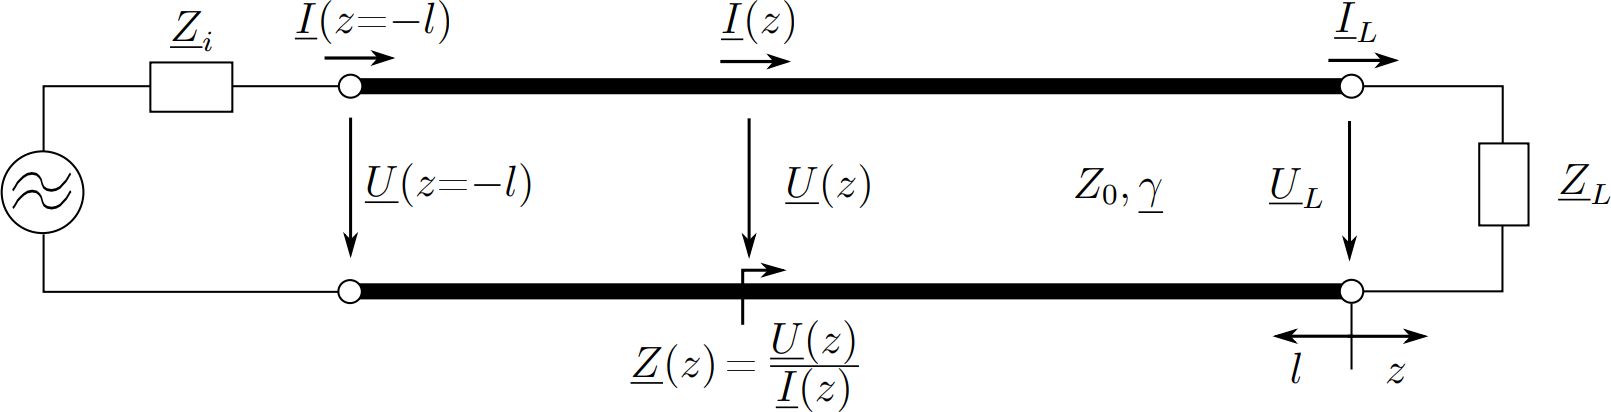
\includegraphics[width=\textwidth]{images/leitung_abschlussimpedanz.png}
\end{figure}
Hier sind Strom und Spannung am Ende der Leitung ($z=0$) bekannt: $\underline{U}(z=0)=\underline{U}_L$ und $\underline{I}(z=0)=\underline{I}_L$.

Mit diesen Randbedingungen lassen sich $\underline{U}_{h0}$ und $\underline{U}_{r0}$ bestimmen:
\begin{equation*}
    \underline{U}(z=0) = \underline{U}_{h0} + \underline{U}_{r0} = \underline{U}_L
\end{equation*}
\begin{equation*}
    \underline{I}(z=0) = \frac{1}{Z_0} (\underline{U}_{h0} - \underline{U}_{r0}) = \underline{I}_L
\end{equation*}

\begin{align}
    \implies \underline{U}_{h0} &= \frac{1}{2} (\underline{U}_L + Z_0 \underline{I}_L)\\
    \implies \underline{U}_{r0} &= \frac{1}{2} (\underline{U}_L - Z_0 \underline{I}_L)
\end{align}

Einsetzen in \eqref{eqn:u-uberlagerung} ergibt
\begin{equation}
    \underline{U}(z) = \underbrace{ \frac{1}{2} \underline{U}_L \left( 1 + \frac{Z_0}{\underline{Z}_L} \right) e^{-\underline{\gamma}z} }_{\text{Hinlaufend}} + \underbrace{ \frac{1}{2} \underline{U}_L \left( 1 - \frac{Z_0}{\underline{Z}_L} \right) e^{\underline{\gamma}z} }_{\text{Rücklaufend}}
    \label{eqn:u-uberlagerung-z}
\end{equation}

\subsection{Reflexionsfaktor}
Der \emph{Reflexionsfaktor $r$ an Stelle $z$} ist definiert als
\begin{equation}
    \tag{Reflexionsfaktor}
    \underline{r}(z) := \frac{\underline{U}_r(z)}{\underline{U}_h(z)} = - \frac{\underline{I}_r(z)}{\underline{I}_h(z)}
\end{equation}
Mit \eqref{eqn:u-uberlagerung-z} und $z=-l$ ergibt sich
\begin{equation}
    \underline{r}(l) = \frac{\underline{Z}_L-Z_0}{\underline{Z}_L+Z_0} e^{2\underline{\gamma}z} = \underline{r}(0) e^{-2\underline{\gamma}l}
\end{equation}
Beziehungsweise:
\begin{equation}
   \underline{r}(l) = \frac{\underline{Z}(l)-Z_0}{\underline{Z}(l)+Z_0} 
\end{equation}
\noindent
Für verlustlose Leitungen wird zusätzlich der \emph{SWR} definiert:
\begin{equation}
    \tag{VSWR}
    s := \left| \frac{\underline{U}_\text{max}}{\underline{U}_\text{min}} \right|
\end{equation}
Das Inverse davon nennt man \emph{Anpassungsfaktor}:
\begin{equation}
    \tag{Anpassungsfaktor}
    m := \frac{1}{s}
\end{equation}

\subsection{Sonderfälle}
\begin{enumerate}
    \item \emph{Anpassung} ($Z_L = Z_0$)\\
        $\underline{r} = 0$
    \item \emph{Leerlauf}
    \item \emph{Kurzschluss}
    \item \emph{$Z_L$ rein imaginär}
    \item \emph{$l = \frac{\lambda}{4}$}
    \item \emph{$l = \frac{\lambda}{2}$}
\end{enumerate}



\chapter{Smith-Diagramm}

\chapter{Streumatrix}

\chapter{Rauschen}

\chapter{Komponenten}

\chapter{Übertragungssysteme}

\chapter{Modulation}

\chapter{Wellenausbreitung}

\end{document}

